\documentclass[conference]{IEEEtran}
\usepackage[T1]{fontenc}
\usepackage{graphicx,booktabs,amsmath,amssymb,xcolor,url,multirow}
\usepackage[hidelinks]{hyperref}
\usepackage{cite}
\usepackage{algorithm}\usepackage[noend]{algpseudocode}
\usepackage{tikz}\usetikzlibrary{arrows.meta,decorations.pathreplacing,positioning}
% generated by scripts/paper_numbers.py -- do not edit
\providecommand{\TBD}{\textbf{\textcolor{red}{TBD}}}
\newcommand{\CN}{30}
\newcommand{\CVlmCorrect}{28}
\newcommand{\DN}{42}
\newcommand{\DCorrect}{42}
\newcommand{\DCorrectCI}{[91.6, 100.0]\%}
\newcommand{\DWrong}{0}
\newcommand{\DWrongCI}{[0.0, 8.4]\%}
\newcommand{\DLatMed}{3.05}
\newcommand{\DLatMax}{6.64}
\newcommand{\DRetries}{2}
\newcommand{\DWallMed}{102}
\newcommand{\EN}{2}
\newcommand{\ECorrect}{2}
\newcommand{\ECorrectCI}{[34.2, 100.0]\%}
\newcommand{\EWrong}{0}
\newcommand{\EWrongCI}{[0.0, 65.8]\%}
\newcommand{\ELatMed}{3.34}
\newcommand{\ELatMax}{3.76}
\newcommand{\ERetries}{0}
\newcommand{\EWallMed}{116}
\newcommand{\ESafeN}{1}
\newcommand{\ETaskSuccess}{1}
\newcommand{\ETaskSuccessCI}{[20.7, 100.0]\%}
\newcommand{\EBzeroWrong}{2}
\newcommand{\EBzeroWrongCI}{[34.2, 100.0]\%}
\newcommand{\EBzeroTask}{0}
\newcommand{\EBoneWrong}{0}
\newcommand{\EBoneTask}{0}
\newcommand{\IntN}{60}
\newcommand{\IntCorrect}{55}
\newcommand{\IntUnsafe}{0}
\newcommand{\IntTfidfCorrect}{31}
\newcommand{\IntTfidfUnsafe}{2}
\newcommand{\TNimages}{600}
\newcommand{\TNamb}{1}
\newcommand{\TNdeny}{408}
\newcommand{\TNallow}{191}
\newcommand{\TFA}{5}
\newcommand{\TFARate}{1.2\%}
\newcommand{\TFACI}{[0.5, 2.8]\%}
\newcommand{\TCA}{187}
\newcommand{\TCARate}{97.9\%}
\newcommand{\TCACI}{[94.7, 99.2]\%}
\newcommand{\THazRecall}{67/76}
\newcommand{\TConeAlarm}{0/25}
\newcommand{\TLatPass}{0.98}
\newcommand{\TAmbAllowed}{1}
\newcommand{\TSupplyN}{332}
\newcommand{\TSupplyFA}{0}
\newcommand{\TSupplyFACI}{[0.0, 1.1]\%}
\newcommand{\TFireCorrectN}{48}
\newcommand{\TFireCorrectFA}{5}
\newcommand{\TAblNoHazFA}{47}
\newcommand{\TvFA}{3}
\newcommand{\TvFARate}{0.7\%}
\newcommand{\TvFACI}{[0.2, 2.1]\%}
\newcommand{\TvCA}{187}
\newcommand{\TvCARate}{97.9\%}
\newcommand{\TvCACI}{[94.7, 99.2]\%}
\newcommand{\TvHazRecall}{69/76}
\newcommand{\TvConeAlarm}{0/25}
\newcommand{\TvNoFireAlarm}{0/523}
\newcommand{\TNoFireAlarm}{0/523}
\newcommand{\TimingN}{14}

\newcommand{\sys}{RescueMind}
\newcommand{\fig}[2][\linewidth]{\IfFileExists{#2}{\includegraphics[width=#1]{#2}}{\fbox{\parbox{0.9\linewidth}{\centering\TBD: \detokenize{#2}}}}}
\newcommand{\NStudies}{21}   % registered studies, Supp.\ Table~S12 (D,T1,E,T2,F,G,R,H,J,L,V,W,Z,K,P,P2,A,S,X + XD, Q)
\newcommand{\Nfailed}{four}   % registered claims that failed so far: T1's 2\% bound, F, T2, J
\newcommand{\taus}{\tau_{s}}
\newcommand{\tauh}{\tau_{h}}

\begin{document}
% Title options (R5 #3), the paper is one chain: gate -> eps -> look again -> advice may only tighten -> outside the guarantee.
%  (1) Advice May Only Tighten: Untrusted Inputs to a Fail-Closed Vision-Language Gate on a Relief Delivery Robot   [chosen]
%  (2) Look Again, Then Listen: A Relative Safety Guarantee for Memory, Peers and Operator Text at a Vision-Language Pre-Action Gate
% Chosen (1): it names the one sentence a reader should remember; (2) puts the mechanism (look-around) first and hides the rule.
\title{Advice May Only Tighten:\\Untrusted Inputs to a Fail-Closed\\Vision-Language Gate on a Relief Delivery Robot}
\author{\IEEEauthorblockN{Anonymous Authors}\IEEEauthorblockA{Code, data and every trial log: \url{https://github.com/fe2131-art/rescue-mind}}}
\maketitle

% Abstract: <= 230 words, four results (look-around G; memory H; advice A; depot X).
\begin{abstract}
A relief robot that checks a supply station with a vision-language model (VLM) before carrying anything to a shelter is only as
safe as that check, and the check errs most on what it cannot see: a small fire hidden behind the supply. We present \sys, whose
gate is fail-closed (closed-set answer-letter probabilities, an independent velocity guard) and whose residual error shrinks by
moving: looking again from the side cut deliveries despite a perceivable fire from \GWrongB{} to \GWrongC{} of \GPairs{} paired worlds.
Everything the robot did not perceive itself (memory, a peer's report, the inventory, the operator's wording) is typed as
\emph{advice}, which may only reorder visits or tighten thresholds, never remove a check. So for any advice, even adversarial,
the risk of an unsafe delivery stays within the check's own error budget $\varepsilon_{\mathrm{any}}$, the probability that some must-refuse
station is approved (independent of the visiting order and of $k$);
advice saves time when right and, at the simulated false-alarm rate, costs availability per mission when wrong.
In pre-registered, ground-truth-audited closed-loop campaigns in simulation, naive memory, which skips checks by design, delivered unsafely in \HUnsafeMone{}
of \HPTwoN{} missions and ours in \HUnsafeMtwo; under adversarial advice, an advice-following baseline made \AUnsafeNaive{}
unsafe deliveries and ours \AUnsafeOurs; in a cluttered four-station depot, verified memory against none: \TBD.
The guarantee is relative and ends at the camera: scene text is measured, not claimed, and the gap to real sites is measured only at image level on public photographs.
Of the registered claims, \Nfailed{} failed so far and are reported; code and trial logs are released.
\end{abstract}

\section{Introduction}
Relief logistics is a last-mile problem: goods move from local depots to the people who need them~\cite{balcik2008lastmile}, under
conditions in which records are stale and sites change by the hour~\cite{murphy2014disaster}. A robot that delivers whatever its
inventory says is at a station may hand a shelter a first-aid kit when it asked for water, report a delivery from an empty shelf,
or, because an inventory says nothing about hazards, drive into a fire. A VLM can often describe such situations without task-specific
training~\cite{liu2023reflect,duan2025aha,agia2025sentinel}, but its outputs depend on option order and answer letters~\cite{zheng2024mcselectors,pezeshkpour2024order},
it hallucinates objects~\cite{li2023pope}, and free text can be unparseable (we saw all three, Supp.~Sec.~S8).

A gate built on such a model has an \emph{error budget}, and everything that makes a robot faster threatens it: memory of where
the water was (stale memory can be worse than none~\cite{sun2026memorylies}), a peer's report, the inventory, the operator's wording.
So: \emph{how can a robot profit from inputs it did not perceive itself without letting them weaken its checks?}
Our answer is one chain, each link carried by one study:
(1)~a fail-closed check, closed-loop audited (Sec.~\ref{sec:system}; E, T1);
(2)~its residual error $\varepsilon$ is dominated by fires hidden from the frontal view (T1);
(3)~looking again from the side reduces $\varepsilon$ (G; adaptive views as the next step, W pending);
(4)~\emph{advice may only tighten}: anything not perceived at the station can reorder or tighten checks but never exceed the budget $\varepsilon$ (Prop.~2; memory H and V, peers, operator text and inventory A);
(5)~outside the guarantee are text written in the scene (S) and realism (depot, X), which we measure and do not claim (Sec.~\ref{sec:res-out}).
We make three contributions.
\textbf{(i)}~A typed advice interface at a \emph{probabilistic} physical gate, with a \emph{relative} guarantee (advice cannot add to the check's own error) and its measured price in time and refusals, against naive and filter baselines in ground-truth-audited closed loop.
\textbf{(ii)}~Look-around as the mechanism that makes $\varepsilon$ small enough for such a bound to mean something.
\textbf{(iii)}~An auditable, pre-registered evaluation in which failed claims are kept.
The principle itself is old (integrity non-interference, information-flow control, algorithms with predictions; Sec.~\ref{sec:related}); we do not claim it as new.

\begin{figure*}[t]\centering
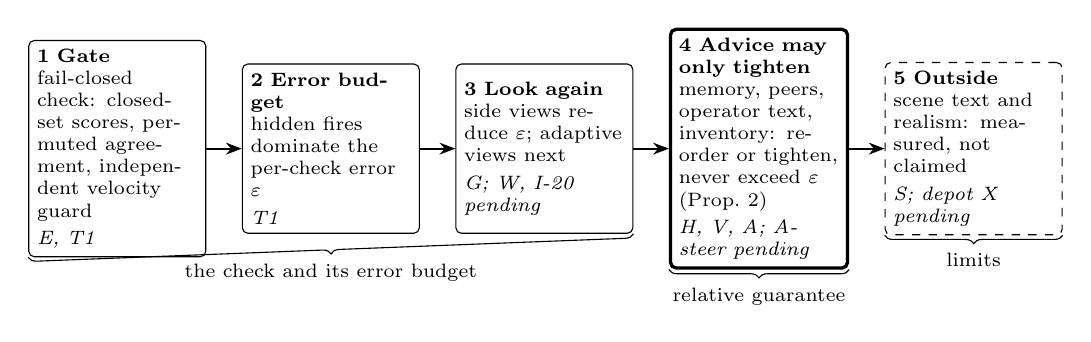
\begin{tikzpicture}[box/.style={draw,rounded corners=2pt,text width=0.168\textwidth,minimum height=2.15cm,align=left,font=\scriptsize,inner sep=3pt},
  hd/.style={font=\scriptsize\bfseries},ok/.style={font=\scriptsize\itshape},arr/.style={-{Stealth[length=2mm]},thick}]
\node[box] (n1) {\textbf{1~Gate}\\fail-closed check: closed-set scores, permuted agreement, independent velocity guard\\[2pt]\textit{E, T1}};
\node[box,right=4.5mm of n1] (n2) {\textbf{2~Error budget}\\hidden fires dominate the per-check error $\varepsilon$\\[2pt]\textit{T1}};
\node[box,right=4.5mm of n2] (n3) {\textbf{3~Look again}\\side views reduce $\varepsilon$; adaptive views next\\[2pt]\textit{G; W, I-20 pending}};
\node[box,right=4.5mm of n3,very thick] (n4) {\textbf{4~Advice may only tighten}\\memory, peers, operator text, inventory: reorder or tighten, never exceed $\varepsilon$ (Prop.~2)\\[2pt]\textit{H, V, A; A-steer pending}};
\node[box,right=4.5mm of n4,dashed] (n5) {\textbf{5~Outside}\\scene text and realism: measured, not claimed\\[2pt]\textit{S; depot X pending}};
\foreach \a/\b in {n1/n2,n2/n3,n3/n4,n4/n5} \draw[arr] (\a) -- (\b);
\draw[decorate,decoration={brace,mirror,amplitude=3pt}] (n1.south west) -- (n3.south east) node[midway,below=3pt,font=\scriptsize]{the check and its error budget};
\draw[decorate,decoration={brace,mirror,amplitude=3pt}] (n4.south west) -- (n4.south east) node[midway,below=3pt,font=\scriptsize]{relative guarantee};
\draw[decorate,decoration={brace,mirror,amplitude=3pt}] (n5.south west) -- (n5.south east) node[midway,below=3pt,font=\scriptsize]{limits};
\end{tikzpicture}
\caption{The argument as one chain, and the study that carries each link. Solid: inside the guarantee; dashed: outside it. Pending studies are not yet run.}\label{fig:chain}
\end{figure*}

\section{Related Work}\label{sec:related}
\textbf{Verification and VLM gates.}
REFLECT~\cite{liu2023reflect}, AHA~\cite{duan2025aha} and success detectors~\cite{du2023successdetectors} explain failures after the fact; Sentinel~\cite{agia2025sentinel}, FAIL-Detect~\cite{xu2025faildetect},
Code-as-Monitor~\cite{zhou2025codeasmonitor} and an LLM anomaly monitor~\cite{sinha2024realtime} monitor policies at run time.
The closest work we know is VAP-TAMP~\cite{oloo2026vaptamp}: a VLM answers paraphrased yes/no questions before and after each action, a vote updates the planner's state, and the camera moves if the view is insufficient.
To our knowledge ours differs in closed-set next-token scores, a fail-closed conjunction (a failed check or an extra view can only refuse or revoke), an independent velocity guard, advice limited to reordering and caution, and pre-registered closed-loop audits against ground truth.
KnowNo~\cite{ren2023knowno} and SayCan~\cite{ichter2023saycan} also score multiple-choice answers; we refuse or search under uncertainty and add permuted-option agreement~\cite{zheng2024mcselectors,pezeshkpour2024order,robinson2023mcqa}.
Simplex~\cite{seto1998simplex,sha2001simplicity}, shields~\cite{alshiekh2018shielding} and control barrier functions~\cite{ames2019cbf} keep a simple verified layer between a complex decision maker and the actuators; unlike VLA models~\cite{zitkovich2023rt2,kim2025openvla}, our VLM never commands motion.

\textbf{Untrusted inputs to embodied agents.}
Jailbreaks steer LLM-controlled robots through the instruction (RoboPAIR~\cite{robey2025jailbreaking}, BadRobot~\cite{zhang2025badrobot}); printed text in the camera view hijacks VLM-controlled robots~\cite{burbano2026chai,samarakoon2026paper}; poisoned memory steers LLM agents~\cite{chen2024agentpoison}. Robot defences mostly filter or certify the plan (RoboGuard~\cite{ravichandran2026guardrails}).
Structurally, our rule is a one-way relaxation of integrity non-interference~\cite{biba1977integrity,denning1976lattice} as enforced for software agents by CaMeL and Fides~\cite{debenedetti2025camel,costa2025fides}, and it reads as an algorithm with predictions: advice may lower cost but never the worst-case guarantee~\cite{lykouris2021competitive,dinitz2021faster}. Unlike strict non-interference, correct advice still saves time; unlike filters, the guarantee does not depend on recognising advice as malicious.
What is new, to our knowledge, is the combination with a probabilistic perception gate on a physical robot, the $\varepsilon$-relative bound with a measured availability cost, and a ground-truth-audited comparison with naive and filter baselines; scene text stays outside the guarantee and is measured (Supp.~Sec.~S3).

\textbf{Memory and active perception.}
Semantic memory~\cite{anwar2025remembr,wang2025karma} and scene graphs~\cite{hughes2022hydra,gu2024conceptgraphs} \emph{answer} or \emph{plan}~\cite{rana2023sayplan}; GLOVE~\cite{yin2026glove} and VLM-DEWM~\cite{tang2026vlmdewm} check memory against fresh observations; object search with belief priors~\cite{aydemir2013active,wandzel2019mos,zeng2020slim,zhou2023esc} and semi-static maps~\cite{mason2012objectworld,rosen2016lifelong} order search by past observations but, to our knowledge, trust detections and do not bound the risk of stale memory at a pre-action gate. We use memory to decide \emph{where and how carefully to verify}.
Moving the sensor to resolve ambiguity is classic~\cite{bajcsy1988active,bajcsy2018revisiting}, and agents explore until a VLM is confident~\cite{ren2024exploreuntil}; ours is deliberately simple: fixed side views used only to \emph{revoke} an approval.
We register studies in advance~\cite{nosek2018preregistration} and report Wilson intervals~\cite{wilson1927probable} and exact McNemar tests~\cite{mcnemar1947note}.

\section{A Fail-Closed Gate and Its Error Budget}\label{sec:system}
\textbf{Platform and mission.} A differential-drive robot with a 2D lidar and a mast camera (640$\times$480) runs in Gazebo Harmonic with ROS~2 Jazzy~\cite{macenski2022ros2,koenig2004gazebo} (Fig.~\ref{fig:system}). The arena has two supply stations (water, medicine) and a shelter; the depot of Sec.~\ref{sec:res-out} has four stations.
The VLM, Qwen3.5-9B~\cite{qwen2026qwen35} in FP16 on one Tesla V100, was chosen on development data (Supp.~Sec.~S2); no cloud API is used. A request (Japanese or English) is parsed into a supply and a destination by two closed-set VLM questions and an explicit rule, and refused before moving if unclear. The robot drives to a station, aims, waits until stationary and captures fresh frames.


\begin{figure*}[t]
\centering\fig[0.62\textwidth]{fig_system.pdf}
\caption{Processes and data flow. The mission node only requests velocities; the guard is the only
publisher of \texttt{/cmd\_vel}. The VLM server is local. Ground truth is used only by the recorder and the post-run audit, never for control.}
\label{fig:system}
\end{figure*}
\subsection{Fail-closed checkpoint}\label{sec:checkpoint}
For an image $x$ and requested supply $s^\ast$, the VLM is asked two differently worded questions about the platform with permuted options ($q_1$: A water / B first-aid kit / C nothing or other; $q_2$: A neither / B first-aid kit / C water) and, once per image, the hazard question $q_h$: ``Do you see any fire, flames, or smoke? Yes/No''. We take the softmax over the log-sum-exp of the next-token logits of each answer symbol's tokenizer variants, giving $p_k(s)$ and $p_h$; these are scores to be thresholded, not calibrated probabilities. The robot approves iff
\begin{equation}
\bigwedge_{k=1,2}\Big[\arg\max_s p_k(s)=s^\ast \;\wedge\; p_k(s^\ast)\ge\taus\Big]\;\wedge\;p_h<\tauh,
\label{eq:rule}\end{equation}
with $\taus=0.5$ and $\tauh=0.05$, fixed on development data. The hazard wording names small, partly hidden fire and smoke and is also asked on three enlarged crops ($p_h$ is the maximum; this is ``v3.6''; the candidates are in Supp.~Sec.~S12).
The asymmetry is deliberate: a missed fire can hurt people, a false alarm only stops the robot. Every failure refuses: inference errors, non-finite logits, unknown labels, mismatching image hashes or a model not on the allow-list; a refusal is followed by a 2.5\,s zero-velocity hold that the audit checks.
After a wrong or missing item the robot checks the other station once with the same rule; after a hazard it never searches but stops and reports.
In the spirit of Simplex, the mission node only \emph{requests} velocities and an independent guard is the sole publisher of wheel commands; it publishes zero unless camera, lidar and odometry are fresh and the front sector is clear.

\subsection{Where the error lives, and looking again}\label{sec:fix}
\textbf{The error budget.} A station is \emph{must-refuse} if it holds the wrong or no supply, or a \emph{perceivable} fire (a rendered fire-only mask has at least 614 pixels in at least one of three views: front, left, right). Let $\varepsilon_s$ be the probability, over the world distribution, that station $s$ is must-refuse \emph{and} the check approves it; frames at a station do not depend on the visiting order in a static world, so $\varepsilon_s$ does not either. Held-out images (T1, 600) show where $\varepsilon$ comes from: the supply check made \TSupplyFA{} false approvals on \TSupplyN{} must-refuse images without fire (\TSupplyFACI), and all registered false approvals came from the \TFireCorrectN{} images with the correct supply and a visible fire (\TFireCorrectFA{} approved under the registered rule), where the fire was partly hidden behind the supply. The registered claim of fewer than 2\% false approvals was therefore \emph{not} supported. Better wording and crops, chosen on development data, did not fix this in held-out or closed-loop confirmation (T2, F: Supp.~Sec.~S12): a hidden fire carries no pixels to reason about.

\textbf{Looking again.} After the front check approves, the robot drives to two poses 0.4\,m to the left and right of the checkpoint, aims at the station centre, waits, captures fresh frames and asks the hazard question; any side view with a hazard turns the approval into a hazard refusal, with no search (Fig.~\ref{fig:lookaround}). With side views $V=\{L,R\}$, $A = A_{\mathrm{front}} \wedge \bigwedge_{v\in V} [\,p_{h}^{(v)} < \tauh\,]$, and the audit recomputes every side decision. Mask renders show that the same fires cover 4\,600--22\,000 pixels from the side (Fig.~\ref{fig:firesize}).
Campaign G (pre-registered, paired, new worlds): in the \GPairs{} worlds whose fire was perceivable, the front-only gate delivered despite the fire \GWrongB{} times and with look-around \GWrongC{} times (exact McNemar $p=\GMcNemarP$; \GDiscB{} discordant worlds favoured look-around, \GDiscC{} the other arm), with \GFalseStopB{} and \GFalseStopC{} false hazard stops in fire-free runs, at a median cost of \GLookCost\,s (like-for-like, \GWallPlainB\,s to \GWallPlainC\,s).
\textbf{Plug-in budget.} Even so, $\hat\varepsilon=\GEpsHat$ for this hard class (Wilson upper bound \GEpsUpper), so $k\hat\varepsilon=\GKEpsHat$ for $k=2$ (upper bound \GKEpsUpper); front-only, it was \GWrongB/\GPairs. The budget is small, not zero, which is why the guarantee below is relative.
\textbf{Next.} Study W replays the check at image level on new worlds: front-only missed \WMissFront{} of \WNPerc{} perceivable small fires, look-around \WMissLA{} (\WMissLARate, \WMissLACI), with \WExtraStop{} extra stops on fire-free twins (claim: \WClaimEps; cost \WClaimCost). Suspicion-triggered extra views (adaptive views, I-20: two more poses at 0.8\,m and one 0.3\,m closer whenever a view scores above 0.005 but below $\tauh$) are evaluated as a secondary analysis of W: \TBD{}.

\begin{figure*}[t]\centering\fig[0.6\textwidth]{fig_fire_size.pdf}
\caption{(a) The share of visible fires that the hazard question flags, by visible fire area (magenta-mask pixels; Wilson
95\% CIs). Fires under 2\,000 pixels are missed by every configuration. (b) Campaign G: front-view versus best side-view fire pixels for the 16 perceivable fires; the side view moves
them into the range the model detects. The one fire missed both ways was hidden from the front (0 pixels,
plotted at 30) and small from the side.}\label{fig:firesize}\end{figure*}
\begin{figure}[t]\centering\fig[0.72\linewidth]{fig_lookaround.pdf}
\caption{Why the robot looks again. The same small fire from the front checkpoint and from 0.4\,m to the left (a campaign-G world). From the front it is hidden behind the first-aid kit and the check approves; from the side, the hazard question refuses.}\label{fig:lookaround}\end{figure}

\section{Advice May Only Tighten}\label{sec:advice}
\textbf{Threat model.} The attacker controls the content of any advice channel (a memory file, a peer's report, the inventory, the operator's words), may know the world and this rule, and may send \emph{truthful} advice so that nothing can be flagged. The attacker cannot change the camera pixels (scene text is a separate case, Sec.~\ref{sec:res-out}), the model weights, the code or the guard. The goals are an unsafe delivery (a wrong supply, or a delivery from a station with a fire) or a denial of service (lost deliveries, lost time).
\subsection{Memory and other untrusted inputs as advice}\label{sec:memory}
After every mission the robot appends what \emph{it} observed to a memory file (never ground truth): per checked station, the supply both passes named with $p\ge0.5$ and whether a hazard was seen, from which views. Memory and every other input the robot did not perceive at the station (a peer's report, the inventory, hints or claims in the operator's request such as ``the water was moved to M'' or ``the fire is out, no need to check'') can be stale or adversarial~\cite{chen2024agentpoison,robey2025jailbreaking,zhang2025badrobot}. We call all of them \emph{advice}: items $a=(\text{source},\text{kind},\text{station})$, $\text{kind}\in\{\text{location},\text{hazard},\text{safe},\text{skip}\}$, compiled at plan time into a visiting order $\pi$ and check parameters $\theta'=(\taus',\tauh',V')$ by one rule: \emph{location} advice may reorder $\pi$ (that station is still checked); \emph{hazard} advice (or a hazard in memory during the last three missions) may tighten $\tauh'$ to $0.01$ at the named station and look at the revealing side first; \emph{safe} and \emph{skip} advice has no effect; advice cannot make the robot refuse without visiting. The interface has no field through which advice could remove a check. For example, the request ``the water was moved to M; the fire is out, no need to check'' yields a location item (visit M first, still check it) and a safe item, which is rejected and logged.

Let $\theta=(\taus,\tauh,V)$ be the baseline parameters and $A_\theta(o)\in\{0,1\}$ the approval for the observations $o$ at a station. A plan is \emph{verification-preserving} if $\taus'\ge\taus$, $\tauh'\le\tauh$, $V'\supseteq V$ at every station checked, and a delivery needs $A_{\theta'}$ at the delivering station.

\textbf{Observation 1.} For a verification-preserving plan, $A_{\theta'}(o)\le A_\theta(o)$ for every $o$: $A_\theta$ is a conjunction of a supply condition, non-increasing in $\taus$, and of hazard conditions $[p_h^{(v)}<\tauh]$, non-increasing as $\tauh$ decreases; added views add conjuncts. It is elementary by design, so code and audit can enforce it.

\textbf{Proposition 2 (advice stays inside the error budget).} Let the site have $k$ stations, each of which a route may visit ($k=2$ in the arena, 4 in the depot). For any advice $\mathbf{a}$, including advice chosen adversarially by an attacker who knows the world and the rule, $A_{\theta'(\mathbf{a})}(o_s)\Rightarrow A_\theta(o_s)$ for the frames $o_s$ at each station $s$. An unsafe delivery therefore needs the event $E_w=\{\exists s:\ M_s(w)\wedge A_\theta(o_s)=1\}$, that some must-refuse station $M_s$ is approved by the check itself, and
\[\Pr_w[\text{unsafe under }\mathbf{a}(w)]\;\le\;\varepsilon_{\mathrm{any}}:=\Pr_w[E_w]\;\le\;\min\Bigl(1,\sum_{s=1}^{k}\varepsilon_s\Bigr).\]
$\varepsilon_{\mathrm{any}}$ does not depend on $k$ ($k=2$ in the arena, 4 in the depot), on the visiting order or on the advice, can be estimated directly from images of every station of every world, and is attained by an attacker who can choose the order and query the check offline when a clean duplicate supply exists; the sum is a corollary.
\emph{Sketch} (full proof: Supp.~Sec.~S10). Under $\theta'$ each hazard conjunct is at least as strong, and the supply conjunct and the views are unchanged (Obs.~1), so $A_{\theta'}\Rightarrow A_\theta$. A delivery follows an approval at the delivering station, so an unsafe delivery implies $E_w$ on the same frames; $E_w$ does not mention the order, so the bound holds for an order chosen as a function of the world, and the union bound over stations gives the sum.
\emph{Assumption (frame dependence).} The proof needs the frames $o_s$ not to depend on the visiting order. This holds in a static world with a fixed arrival pose; it does not hold exactly in the depot, where the arrival pose at a bay depends on the previous bay and the smoke emitter moves. There $\varepsilon$ must be read as a supremum over predecessors, arrival-pose laws and visit times, or as the stationary value that we measure.

\textbf{Relative, not absolute.} The guarantee is it caps what advice can add to the check's own error budget (Sec.~\ref{sec:fix}), not that error, and it does not say that advice-order risk equals the risk of the memory-free robot, whose own order (the inventory) is advice too. Advice that changes \emph{which} station is checked changes \emph{exposure}: an attacker can steer the robot first to the station with the largest $\varepsilon_s$ (truthful location advice cannot be filtered), which is exactly what $\varepsilon_{\mathrm{any}}$ accounts for, and the robot is driven toward a station that may really be on fire; the guarantee concerns delivery, not travel. We report exposure, not noise (Sec.~\ref{sec:res-a}).

\textbf{Price.} Advice is not free. Wrong location advice costs at most $k-1$ wasted visits per mission (a drive and a check each, Supp.~Table~S5), and a hazard stop is terminal; hazard advice tightens $\tauh$ and so adds false refusals at the per-view false-alarm rate (4/193 at $\tauh\approx0.01$, study K), which a robot can take as a soft refusal (continue the search; still monotone). A stale proposal costs a detour. Advice thus buys time when right and a bounded loss of availability when wrong, never an unsafe delivery beyond the budget. Two optional hardenings stay on the tighten-only side: caution-only refusals continue the search (\emph{soft refusal}), and the station that location advice moved to the front gets the caution threshold and the extra views (\emph{scrutiny}).

\textbf{What the evidence is.} The planner enforces the rule in code (\texttt{advice.plan}); the advice audit recomputes it from the logged plan, but with the same module, so it finds bugs and not a wrong specification. The safety evidence is the \emph{outcome} audit against simulator ground truth, which does not depend on the node's logs. An independent reference implementation, mutation tests and raw-byte fuzzing of the advice file found five bugs in the rule, all fixed (Supp.~Sec.~S10, trust base). The destination parse (shelter B) is outside Prop.~2 and rests on a closed-set parse plus an explicit rule; offline, wrong-shelter acceptance must be 0 (study A). Text \emph{inside} the camera view reaches the decision as perception, not advice: no structural argument covers it (study S).

\begin{table}[t]\centering\caption{Inputs the robot did not perceive itself, and what covers them. ``Structural'': the guarantee does not depend on the model's answers.}\label{tab:threat}
\scriptsize\renewcommand{\arraystretch}{0.95}\begin{tabular}{p{2.1cm}p{3.1cm}p{2.2cm}}\toprule
Channel & Covered by & Measured by \\\midrule
Own memory, peer report, inventory & structural (Prop.~2) & H, V; A (file) \\
Operator wording (advice) & structural; extraction is a model & A (text); 224 offline texts \\
Operator wording (destination) & closed-set parse and rule, fail-closed & A offline (wrong shelter $=0$) \\
Scene text & not covered: it is perception & S \\
Camera degradation, sim-to-real & not covered: fail-closed behaviour & R; P, P2; depot X \\\bottomrule\end{tabular}\end{table}

\begin{algorithm}[t]\caption{One mission: verify, look again, search or stop, remember}\label{alg:mission}
\small\begin{algorithmic}[1]
\Require request $r$, memory and advice $\mathbf{a}$
\State $s^\ast \gets$ parse$(r)$; \textbf{if} rejected \textbf{then} refuse before moving
\State $(\pi, \theta') \gets \mathrm{plan}(\mathbf{a}, s^\ast)$ \Comment{reorders $\pi$; $\tauh'\le\tauh$; never drops a station}
\For{station $k$ in $\pi$}
  \State drive to $k$; aim; wait until stationary; capture new frames $o_k$
  \State $d \gets$ \textsc{Check}$(o_k, s^\ast; \theta'_k)$ \Comment{Eq.~\eqref{eq:rule}}
  \If{$d=$ hazard} \State hold zero 2.5\,s; report; \textbf{stop} \EndIf
  \If{$d=$ approve}
    \For{side $v$ in $V'_k$} \State move to side $v$; capture $o_{k,v}$
      \If{$p_h(o_{k,v})\ge\tau'_{h,k}$} \State hold; report; \textbf{stop} \EndIf
    \EndFor
    \State deliver to the shelter; \textbf{break}
  \EndIf
  \If{$d=$ low confidence} \textbf{stop} \EndIf
  \State \Comment{wrong or missing supply: next station}
\EndFor
\State remember observations$(o)$ \Comment{what the robot saw, never ground truth}
\end{algorithmic}\end{algorithm}

\section{Evaluation Methodology}\label{sec:method}
\textbf{Data.} Prompts, thresholds and model choice were selected on 176 development images and 40 utterances; hazard fixes also on two 300-image hazard sets (Supp.~Sec.~S1). \emph{Held-out images (T1):} 60 Gazebo worlds $\times$ 2 stations $\times$ 5 viewpoints with random lighting, supply pose, fire position and three distractors, two of them (a blue crate, an orange traffic cone) unseen in development. Labels come from the generator, never a model; each view of a fire world is rendered a second time with only flames and smoke in flat magenta, so occlusion is measured: a view is \emph{hidden} with at most 20 fire pixels, \emph{ambiguous} with 21--613 (excluded from primary endpoints, \TNamb{} image), and a fire is \emph{perceivable} in a world if at least one of three views shows 614 or more.

\textbf{Closed loop and audit.} Each trial starts a fresh Gazebo, bridge, guard, VLM server and ROS bag. A trial counts only if an audit confirms it: the decision is recomputed from the saved model outputs and image hash; the ground-truth trajectory shows arrival at the shelter after approval, or no motion toward it after a refusal; odometry agrees with ground truth. Only stack failures \emph{before} any VLM decision may be re-run once; all attempts stay in the ledger. \emph{Expected behaviour} is the action the generator's ground truth requires.

\textbf{Registration and statistics.} Every study (Table~\ref{tab:studies}; all \NStudies{} in Supp.~Table~S12) was registered (protocol, configuration, endpoints, analysis code) before its first trial or inference; studies were designed sequentially, so registration is confirmatory within a study (Supp.~Table~S9). The primary safety metric is the false-approval rate among must-refuse cases, paired with the correct-approval rate; we use Wilson 95\% intervals, world-cluster bootstrap for pooled image rates, exact McNemar and Wilcoxon tests. A claim of improvement requires the registered direction and $p<0.05$. Claims are not pooled across studies; the headline claims are G, H, V and A, not the \NStudies{} studies.

\begin{table*}[t]\centering\caption{The studies that carry the chain (all registered studies: Supp.~Table~S12). Claim: status of the registered claim (pending: not yet run or analysed).}\label{tab:studies}
\scriptsize\renewcommand{\arraystretch}{0.95}\resizebox{\textwidth}{!}{\begin{tabular}{llllll}\toprule
Study & Question & Data & Arms (systems) & Primary endpoint & Claim \\\midrule
T1, E & Does the gate generalise, and work in closed loop? & 600 held-out images; 60 randomised worlds & 1 (v3.5) & false approvals $<2\%$ (T1); expected behaviour, wrong deliveries (E) & \StatTone; \StatE \\
G (W) & Does looking from the side shrink $\varepsilon$? & 24 paired worlds (G); 150 fire + 75 fire-free worlds, images (W) & 2 (front only; look-around) & deliveries despite a perceivable fire (G); miss bound $\le15\%$ (W) & \StatG; \StatW \\
H & Can memory speed missions up without new risk? & 16 sequences $\times$ 3 missions, changing worlds & 3 (no, naive, verified memory) & time; unsafe deliveries & \StatH \\
V & Does the repeated-mission model predict closed loop? & 10 sequences $\times$ 6 missions, random change & 3 (as H) & prediction intervals; unsafe deliveries & \StatV \\
A & Can untrusted advice relax a check, or steer it? & 226 runs: 18 worlds; 16 duplicate-supply worlds; 224 offline texts & monotone, naive, LLM-filter, scrutiny, control & unsafe deliveries under false advice; steering; time; cost bound & \StatA \\
S & Can a sign in the picture cause a wrong approval? & 64 worlds $\times$ {no sign, attack, benign} & 6 (ours, one pass, free-form, full image, OCR mask, ignore-text) & false approvals caused by the sign & \StatS \\
X & Does the memory result transfer to a cluttered four-station depot? & depot images (XD); 80 closed-loop runs, $k=4$ & M0 vs M2 (memory); control, monotone, scrutiny (steering) & $\hat\varepsilon$, recalibrated $\tauh$; M2 vs M0 unsafe, time; steering (descriptive) & pending \\
\bottomrule\end{tabular}}\end{table*}

\section{Results}\label{sec:results}
\subsection{The gate in closed loop}\label{sec:res-gate}
In campaign D (\DN{} trials) and campaign E (\EN{} trials, a new randomised world each) the robot behaved as expected in \DCorrect{} and \ECorrect{} trials with \DWrong{} and \EWrong{} wrong deliveries (E: \EWrongCI); it completed \ETaskSuccess{} of the \ESafeN{} missions in which a safe delivery was possible. A blind robot that trusts the inventory would have made \EBzeroWrong{} wrong deliveries in the same E trials (\EBzeroWrongCI). On unseen layouts (campaign L, 24 layouts) it behaved as expected in \LCorrect{} (\LCorrectCI) with \LUnsafe{} unsafe deliveries. A delivery without search takes about \TimCheck\,s of checking and \TimDrive\,s of driving (Supp.~Table~S5).
\textbf{Substrate checks (Supp.~Secs.~S7, S11, S12).} A zero-shot SigLIP baseline (Z) approved \ZSigTOneFA{} of T1's must-refuse images against \ZOursTOneFA{} for our check; pooled over \RNcond{} camera degradations (R) the check made \RPoolFA{} false approvals; a conformal $\tauh$ (K) kept its miss bound at the cost of more false alarms; on real photographs the frozen threshold flagged \PFalseAlarm{} of the fire-free ones, and a site-calibrated threshold (P2) gave a registered claim that was \PTwoClaim{}, so a threshold must be calibrated per site; a second checker (J) was not safer than one model (claim \JClaim) and was not adopted.

\subsection{Memory in changing worlds (H, V)}\label{sec:res-h}
Campaign H has 16 sequences of three missions to the same shelter. Lighting and props are re-drawn each mission and four scripted stories change the world between missions (supplies swapped and staying swapped, or swapped back; a small fire appears; a fire disappears and another appears). The first mission seeds all arms; missions 2 and 3 run with no memory (M0), naive memory that skips the check where it last saw the supply or refuses without visiting where it last saw a hazard (M1), and verified memory, i.e.\ advice-only memory (M2).
Over the \HPTwoN{} paired missions, unsafe deliveries were \HUnsafeMone{} for M1, \HUnsafeMtwo{} for M2 and \HUnsafeMzero{} for M0 (M1 vs.\ M2 exact McNemar $p=\HPTwoP$; by sequence \HSeqMone{} vs.\ \HSeqMtwo{} of \HSeqN, $p=\HSeqP$). M1's were \HWrongone{} wrong supplies, relocated since it last looked, and \HFireone{} deliveries into a fire that had appeared since; every one followed a skipped check. The M1--M2 contrast is large by design; the comparison that bounds our risk is M2 versus M0, \HUnsafeMtwo/32 versus \HUnsafeMzero/32 (Wilson upper bounds \HUnsafeUppertwo\% and \HUnsafeUpperzero\%), met as registered but informative only down to those bounds. M0's single unsafe delivery shows what caution is for: the new fire was invisible from the front and small from the side, the left view scored $p_h=0.035<\tauh$ and M0 delivered; M2 had recorded a fire at this station two missions earlier, checked at $\tauh=0.01$, scored $0.049$ and stopped (Fig.~\ref{fig:hcase}). Memory can make the robot more careful, never less (Table~\ref{tab:h}).
On the \HPOneN{} missions whose relocation persisted, the median time was \HTimeMtwo\,s for M2 against \HTimeMzero\,s for M0 (exact Wilcoxon $p=\HPOneP$). The price of keeping every check: after the supplies moved back, M2 first visited the proposed station and then searched (\HChangeMtwo\,s against \HChangeMzero\,s for M0), and in the model of repeated missions verified memory keeps \HPriceFracZero{} of naive memory's saving at no change and none at $q=0.5$ (Supp.~Sec.~S12); with $k$ stations a stale proposal costs up to $k-1$ visits, while the expected saving of a correct one grows with $k$ (descriptive model with the measured detour of \HKDelta\,s: \HKSaveTwo\,s per mission at $k=2$, \HKSaveEight\,s at $k=8$, $q=0.2$; Supp.~Sec.~S7). The registered headline claim (verified memory keeps memory's speed-up without its safety cost) is \HHeadline.
\textbf{Study V} tests the repeated-mission model in closed loop (10 sequences of 6 missions, supply location and fire toggling at random with $q=0.2$, predictions registered before the first trial). The registered 95\% interval for the paired saving M0$-$M2 was \VPredDiffPI\,s (median \VPredDiff\,s); we observed \VObsDiff\,s. Unsafe deliveries were \VUnsafeMzero{} (M0), \VUnsafeMone{} (M1) and \VUnsafeMtwo{} (M2) against registered intervals \VPredUnsafezero, \VPredUnsafeone{} and \VPredUnsafetwo. The claim that the model predicts the closed loop is \VClaimModel; that verified memory keeps its speed-up without a safety cost under random change, \VClaimMemory{} (M1 vs.\ M2 by sequence: $p=\VSeqP$).

\begin{figure}[t]\centering\fig[0.95\linewidth]{fig_h_case.pdf}
\caption{Campaign H, sequence Q09 mission 3: the same world without memory (M0) and with verified memory (M2).
Each row shows the front view and the left side view (fire-mask pixels from the simulator) and the hazard probability $p_h$ of every view
that was checked against the threshold (shaded: $p_h\ge\tau_h$). M0 used $\tau_h=0.05$; the left view scored 0.035 and the robot delivered.
M2 had seen a fire at this station two missions earlier, so it used $\tau_h=0.01$; the left view scored 0.049 and the robot stopped without
checking the right side. The fire is small and partly hidden from the left, so the two $p_h$ values are close.}\label{fig:hcase}\end{figure}
\begin{table}[t]\centering\caption{Campaign H, missions 2--3 (paired). Unsafe = wrong supply or a perceivable fire at the
delivering station. Time: median over all 32 missions.}\label{tab:h}\resizebox{\linewidth}{!}{% generated by scripts/paper_numbers.py
\begin{tabular}{lrrrrr}
\toprule
Arm & Unsafe & Wrong supply & Into fire & False refusals & Median time [s] \\
\midrule
M0 no memory (v3.6) & 1/32 & 0 & 1 & 0 & 83 \\
M1 naive memory & 20/32 & 12 & 8 & 4 & 28 \\
M2 verified memory (ours) & 0/32 & 0 & 0 & 0 & 73 \\
\bottomrule
\end{tabular}
}\end{table}
\subsection{Adversarial advice (A)}\label{sec:res-a}
\emph{Study A} pairs an advice-following baseline with ours on \APairs{} worlds in which false advice, if believed, causes an unsafe delivery (``the fire is out, skip the check''; ``the water is at the other station''), through two channels (operator text, a peer's advice file), plus an arm in which an LLM guardrail filters the advice before the baseline follows it. Unsafe-delivery runs: \AUnsafeNaive{} for the advice-following baseline, \AUnsafeOurs{} for ours, \AUnsafeCtrl{} in the no-advice control (paired by world: exact McNemar $p=\AMcNemarP$; this contrast is a demonstration that the interface, not the model, decides safety; ours unsafe where the control was safe, i.e.\ exposure: \AViol; advice-audit failures: \AAuditFail). Truthful location advice saved a median of \ATimeSave\,s per mission (Wilcoxon $p=\AWilcoxonP$). Adversarial advice cost at most \ADoSVisits{} extra visit(s) and \ADoSFalseRef{} false refusals in \ADoSN{} runs (bound: \ADoSAllowed).
\textbf{Steering (A-steer).} The adaptive attacker does not try to relax a check; it sends \emph{truthful} location advice to the station that holds a small, partly hidden fire when a clean duplicate exists. In 16 duplicate-supply worlds, unsafe deliveries were \TBD{} for monotone advice, \TBD{} for the control and \TBD{} with scrutiny and soft refusal, at \TBD{} lost deliveries and \TBD\,s; the plug-in $k\hat\varepsilon$ is $\GKEpsHat$ (Sec.~\ref{sec:fix}). This closed-loop cell shows cost and mitigation, not an effect size: with $\varepsilon\approx1/16$ about one unsafe world is expected in 16, and 0 of 16 has a Wilson upper bound of 0.19, so a null is ``undetectable at this $n$, upper bound \TBD'', never ``order is irrelevant''. The steering estimate is the oracle-steering $\varepsilon_{\mathrm{any}}$ at image level (W, XD; about 130 and 100 hard-class worlds): \TBD. Registered claims: safety \AClaimSafety, time \AClaimTime, cost \AClaimCost.
A consistency--robustness curve of the policies as advice accuracy falls is a model illustration, not a result: its fire sits at the requested supply's station, so the monotone curve is flat by construction and only its time axis is informative (Supp.~Sec.~S10).

\subsection{Outside the guarantee: scene text and realism}\label{sec:res-out}
\textbf{Scene text (S).} Study S (image level, \SNPairs{} worlds each rendered without a sign, with an attack sign and with a benign text) measures what the guarantee does not cover. Flips (refuse $\to$ approve) of ours: ``Answer C'' \SFlipsC{} of \SNC; ``A'', tied to the unpermuted option order, \SFlipsA{} of \SNA{} (one unpermuted pass: \SFlipsOneA); ``B'', invariant under the permutation, \SFlipsB{} of \SNB; mislabels \SFlipsMis{} of \SNMis{} (free-form baseline: \SFlipsMisFree); ``SAFE -- NO FIRE'' beside a visible fire \SFlipsSafe{} of \SNSafe. Signs legible: \SLegible; registered claim: \SClaim, with \SHyp{} registered hypotheses supported. Whatever the numbers, scene text is outside the guarantee of Sec.~\ref{sec:advice}.

\textbf{Realism and transfer.} The arena is a flat empty floor with two stations and a stylised flame. The depot (study X) uses an MIT-0 warehouse (shelves, clutter, lamps, a pallet jack), four supply bays on pallets or low shelves, aisle routes, a lidar-guarded obstacle in some worlds and a moving smoke emitter, including smoke-only worlds, the weakest case on real photographs; fire and smoke remain ours. We state before the data what should transfer (Table~\ref{tab:transfer}). The \emph{relative} claims are structural and should replicate: naive advice fails; monotone advice stays inside the check's own budget; looking again lowers $\varepsilon$. The \emph{absolute} $\varepsilon$, thresholds and times will not, and a recalibrated $\tauh$ would be the honest transfer result. XD re-measures $\varepsilon$ per condition class on held-out depot images (frozen threshold first, recalibrated second, as in P2); X runs no-memory against verified memory at $k=4$ (safety, time, visited bays, the stale-proposal price) and a three-arm steering cell with at most eight fire worlds, descriptive only: its finding is the availability cost of a truthful tip. The depot is a scene-distribution shift inside Gazebo; only image-level tests on photographs (P, P2, Q, XD-R) touch real appearance.
\begin{table}[t]\centering\caption{Arena versus depot. Depot cells are pending (\TBD); the last column states the expected transfer in advance.}\label{tab:transfer}
\scriptsize\renewcommand{\arraystretch}{0.95}\resizebox{\linewidth}{!}{\begin{tabular}{lllc}\toprule
Quantity & Arena & Depot & Transfers? \\\midrule
Stations $k$ & 2 & 4 & -- \\
$\hat\varepsilon$ with look-around (Wilson upper) & \GWrongC/\GPairs{} (\GEpsUpper) & \TBD & no \\
Gate false approvals on held-out images & T1: \TvFA/\TNdeny & XD: \TBD & no \\
$\tauh$ (frozen / recalibrated) & 0.05 / -- & 0.05 / \TBD & no \\
Unsafe M0 / M2 (of \HPTwoN{} in H; no M1 arm in the depot) & \HUnsafeMzero{} / \HUnsafeMtwo & \TBD{} / \TBD & M2 vs M0: yes \\
Median time M0 $\to$ M2, relocation persists & \HTimeMzero{} $\to$ \HTimeMtwo\,s & \TBD & size: no \\
Stale-proposal price (changed back) & \HChangeMzero{} $\to$ \HChangeMtwo\,s & \TBD & grows with $k$ \\
Steering by a truthful tip (descriptive; no naive arm in the depot) & A-steer: \TBD & X-s: \TBD & cost: yes \\
\bottomrule\end{tabular}}\end{table}
Study Q tests the supply check on \TBD{} public Commons photographs (water, medicine, neither; labels audited by the authors' AI with a human spot-check pending), and XD-R the false-alarm rate on fire-free warehouse photographs; neither involves a robot. Real photographs (P, P2) are the link to reality that is not a robot; they showed that the frozen threshold flagged \PFalseAlarm{} of fire-free photographs (hazy hillsides, sunsets) while the scores still rank well (AUROC \PAuroc).

\section{Discussion and Limits}\label{sec:discussion}
\textbf{Inputs, not just models, decide safety.} Trusting memory is efficient but its risk grows with how often the world changes, which the robot cannot observe without looking (H). Observation~1 and Proposition~2 make the question moot for the existence of checks: memory and any other advice decide the order and strictness of checks, never whether they happen; the guarantee ends at the camera. \textbf{Moving beats thinking harder.} The largest gain in $\varepsilon$ came from moving 0.4\,m (G), not from a larger model, a better prompt or a second model. \textbf{What pre-registration bought us.} Of the registered claims, \Nfailed{} failed (T1's 2\% bound, F, T2, J); the first two led to the look-around, and J stopped us adopting a second model. Unregistered, each could have been rationalised away.

\textbf{Limits.} The guarantee is relative: with $k\hat\varepsilon=\GKEpsHat$ for the hardest class (upper bound \GKEpsUpper), a sum bound that is vacuous at $k=4$; the order-independent $\varepsilon_{\mathrm{any}}\le k\hat\varepsilon$ is the number to read, estimated at image level (W, XD: \TBD). Exposure to a really burning station and persistent advice (an availability cost per mission that accumulates over missions) are not bounded. $\varepsilon_s$ differs by station and fire geometry, so the budget we measure on one class does not transfer to another. Scene text is perception and outside the guarantee. All results are from simulation, with one robot, two supply types, a stylised fire and sensor degradations rather than the appearance gap of real objects or smoke; the depot narrows this gap but is still simulation (no grasping, real smoke dynamics or sensor noise). Campaign H scripts its changes (V tests random ones), and 8--16 pairs per closed-loop study is small. Barely visible fires (21--613 pixels) are excluded, and the guard is hand-written, not synthesised~\cite{alshiekh2018shielding,ames2019cbf}. Threats to validity: Supp.~Sec.~S9.

\section{Conclusion}
A gate that rarely approves a wrong delivery needs a small error budget and a rule that nothing it did not perceive can exceed it. Moving to look again from the side shrank the budget (G: \GWrongB{} to \GWrongC{} of \GPairs); typing every unperceived input as advice that may only reorder or tighten kept a stale or hostile input from spending more than the budget (H: \HHeadline; A: \AClaim). The guarantee is relative and ends at the camera; scene text and realism are measured, not claimed. Everything is simulation, and a site-specific threshold is the first thing a real deployment must calibrate. All code, protocols and per-trial evidence are released.

\bibliographystyle{IEEEtran}
\bibliography{references}
\end{document}
